\documentclass[10pt,twocolumn]{article}

\usepackage[margin=0.75in]{geometry}
\usepackage{amsmath,amssymb,booktabs,microtype}
\usepackage{graphicx}
\usepackage{xcolor}
\usepackage{hyperref}
\usepackage{url}

\hypersetup{
  colorlinks=true,
  linkcolor=blue!60!black,
  citecolor=blue!60!black,
  urlcolor=blue!60!black
}

\newcommand{\pam}{\textsc{PAM}}
\newcommand{\todoexp}[1]{%
  \begin{center}
  \fcolorbox{orange!70!black}{orange!8}{%
    \parbox{0.92\columnwidth}{\textbf{Publication experiment placeholder.} #1}}
  \end{center}}
\newcommand{\placeholderfigure}[2]{%
  \begin{figure}[t]
    \centering
    \fcolorbox{black!55}{black!3}{%
      \parbox[c][#1][c]{0.91\columnwidth}{\centering
        \textbf{Figure placeholder}\\[3pt]#2}}
    \caption{#2}
  \end{figure}}

\title{\textbf{Measuring Memory Independently of Intelligence:}\\
An Intrinsic Probe Suite for Neural Memory Architectures}
\author{Anonymous authors\\
\texttt{Anonymous institution}}
\date{}

\begin{document}
\maketitle

\begin{abstract}
Language-model evaluations usually score behavior that jointly depends on
retention, retrieval, and computation.  A failure therefore does not identify
whether required information was forgotten or merely used incorrectly.  We
propose an intrinsic benchmark that treats a neural memory mechanism as a
dynamical system and measures it before end-task reasoning.  The suite probes
implementation equivalence, associative binding capacity, persistence,
write-induced interference, effective rank, and retrieval over long synthetic
and language-derived streams.  Its synthetic core is deterministic and does
not require a trained checkpoint.  We use Phase-Associative Memory (\pam) only
as a worked case study.  Multi-seed CPU experiments expose capacity, decay,
recency, and constructive-interference effects.  They also show that an
apparent matrix advantage at equal embedding width reverses when HRR receives
the same state-byte budget, illustrating why memory accounting is part of the
benchmark.  These results do not establish trained language-model recall or
downstream superiority; we identify those comparisons as publication
experiments rather than inferring them from mechanism-level measurements.
\end{abstract}

\section{Introduction}
\label{sec:introduction}

Long-context question answering, language modeling, and reasoning conflate at
least three functions: retaining information, retrieving relevant retained
information, and transforming it into an answer.  Benchmarks such as
LongBench, RULER, and BABILong deliberately evaluate useful composed behavior
\cite{bai2023longbench,hsieh2024ruler,kuratov2024babilong}; they do not, by
themselves, identify which internal memory property limited that behavior.
This attribution problem is important when comparing growing attention
caches, fixed-size recurrent states, and fast-weight memories.

We formulate an architecture's memory as a measurable subsystem.  If
\begin{equation}
  S_t = F(S_{t-1},x_t), \qquad y_t = G(S_t,q_t),
  \label{eq:dynamics}
\end{equation}
then the benchmark asks what information remains represented in $S_t$ and can
be recovered by $G$, holding downstream language reasoning outside the core
measurement.  This separation is diagnostic rather than ontological:
memory and computation interact in trained models, and intrinsic scores should
not be read as complete measures of intelligence.

The proposed contribution is the benchmark, not a claim that one memory
architecture is universally best.  Specifically, this paper:
\begin{itemize}
  \item defines a compact set of intrinsic, mechanism-level probes with common
        protocols and explicit capability requirements;
  \item separates associative probes from state-geometry probes, allowing
        unsupported operations to be reported rather than approximated;
  \item provides a deterministic NumPy reference and implementation bridges;
  \item illustrates the measurements on \pam, a complex matrix memory, while
        clearly separating saved mechanism results from deferred trained-model
        experiments.
\end{itemize}

\section{Scope and Evaluation Principle}
\label{sec:scope}

We use ``memory'' operationally: an evolving state that can preserve
information from earlier inputs and make it available later.  An intrinsic
probe supplies controlled writes and reads, or directly inspects the state.
It does not ask the model to interpret an instruction, generate a natural
language answer, or solve a multi-step task.  Behavioral benchmarks remain
necessary because a mechanism with strong intrinsic retention may still be
poorly addressed, trained, or used.

The benchmark has three tiers.  The \emph{associative tier} exposes
\texttt{write}$(k,v)$ and \texttt{read}$(q)$; the \emph{stateful tier} exposes
an update and a two-dimensional view of state for spectral diagnostics.
Matrix fast weights and attention caches support both tiers in the reference
code.  A Mamba state exposes the stateful tier, but no native associative
lookup; associative tests therefore skip it instead of assigning an artificial
score.  This is a current adapter limitation and also a reminder that not all
memory mechanisms share the same native query semantics.  The
\emph{behavioral tier} gives a trained language model controlled textual
associations and scores whether the correct value is available at query time.

\section{Related Work}
\label{sec:related}

\paragraph{Associative and fast-weight memory.}
Holographic Reduced Representations (HRR) bind distributed vectors using
circular convolution \cite{plate1995hrr}.  Fast-weight systems instead modify
a rapidly changing state within a sequence
\cite{schmidhuber1992fastweights,ba2016fastweights}.  Linear attention can be
viewed as a recurrent outer-product memory under an appropriate feature map
\cite{katharopoulos2020linear}.  These traditions motivate controlled
key--value binding tests and explicit interference measurements.

\paragraph{Sequence architectures.}
Attention retains token-indexed key--value pairs but its cache grows with
context length.  Selective state-space models such as Mamba maintain
fixed-size recurrent state and make updates input dependent
\cite{gu2023mamba}.  Our benchmark does not assume that these mechanisms have
identical semantics: it records which probe tier each adapter supports and
compares only well-defined quantities.

\paragraph{Long-context benchmarks.}
LongBench evaluates bilingual, multi-task long-context understanding
\cite{bai2023longbench}; RULER expands synthetic retrieval with multiple
needles, tracing, and aggregation \cite{hsieh2024ruler}; and BABILong embeds
reasoning facts in long natural text \cite{kuratov2024babilong}.  Their target
is end-to-end capability.  Our target is complementary failure attribution:
capacity, decay, interference, and state utilization before language
interpretation and reasoning are introduced.

\paragraph{Reading internal representations.}
The logit lens and tuned lens map intermediate residual states toward output
tokens \cite{nostalgebraist2020logitlens,belrose2023tunedlens}.  Effective rank
summarizes spectral spread and has been used as a continuous alternative to
algebraic rank \cite{roy2007effectiverank}.  Our rank probe is descriptive: a
higher value indicates broader spectral use, not automatically better recall.

\subsection{Relationship to Anthropic's J-space}
\label{sec:jspace}

Anthropic's \emph{Verbalizable Representations Form a Global Workspace in
Language Models} identifies what it calls J-space using an averaged Jacobian
lens \cite{anthropic2026jspace}.  The reported method finds sparse,
token-linked directions in a model's residual stream that are verbalizable
through the output vocabulary.  The study then tests whether those directions
are merely decodable or functionally involved, using causal interventions
across reporting, modulation, reasoning, generalization, and selectivity
experiments.  Its global-workspace interpretation concerns representations
that can be written once and used flexibly by multiple downstream
computations.

That object is related to neural memory, but it is not the object measured
here.  J-space is a representational and causal-interpretability claim about
sparse directions inside a trained language model's residual computation.
Our benchmark evaluates temporal architectural storage: how an explicitly
evolving state binds items, loses them under repeated updates, suffers
cross-talk, uses its available spectrum, and behaves as temporal distance
increases.  A J-space direction can be causally useful without specifying how
the underlying fact survived thousands of state updates; conversely, a memory
state can retain an association without that association entering a
verbalizable workspace.

The methods also differ in their interventions.  The averaged Jacobian lens
links residual directions to token outputs and supports targeted activation
edits.  Our core interventions control writes, keys, values, decay, filler
streams, and query time.  The former asks \emph{which trained internal
representations are available and broadcast}; the latter asks \emph{what a
storage mechanism preserves over time and at what cost}.  Neither result
subsumes the other.

A useful combined experiment would first implant or identify a controlled
fact, then measure (i) its intrinsic survival in the architecture's memory
state and (ii) whether a corresponding verbalizable J-space direction becomes
available to downstream computation.  This could distinguish storage failure,
workspace-access failure, and downstream reasoning failure.  We leave that
combination as future work; no current saved run in this repository measures
J-space.

\section{Benchmark}
\label{sec:benchmark}

\subsection{Common primitives and score}

For the matrix reference, keys and values are unit complex vectors.  A write
and read are
\begin{equation}
  S \leftarrow \gamma S + vk^{*}, \qquad y = Sq,
  \label{eq:write-read}
\end{equation}
where $k^{*}$ denotes conjugate transpose.  Retrieval is normalized against a
fresh single-write state:
\begin{equation}
  \operatorname{rel}(S;k,v) =
  \frac{|\langle Sk,v\rangle|}
       {|\langle(vk^{*})k,v\rangle|+\epsilon}.
  \label{eq:relative}
\end{equation}
This score is an alignment magnitude, not a probability.  Values above one
can occur when later writes align constructively with the queried value.
Top-1 capacity instead compares $y$ against all candidate values.

\subsection{Probe definitions}

\paragraph{Implementation correctness.}
Architectures with parallel training and recurrent inference forms should
satisfy
\begin{equation}
  \max_t \left|y_t^{\mathrm{parallel}}-
                    y_t^{\mathrm{recurrent}}\right| \leq \varepsilon.
\end{equation}
The suite checks supported update modes and bridges the NumPy recurrence to
the implementation layer.  This is a prerequisite, not a memory-quality
score.

\paragraph{Binding capacity.}
Write $N$ independently sampled key--value pairs, query every stored key, and
report top-1 value accuracy as $N$ grows.  The reference comparison is vector
HRR \cite{plate1995hrr}, which binds by circular convolution.  Multiple trials
are required because random cross-talk varies with the sampled dictionary.
We report both equal embedding width and equal state bytes.  The former gives
the matrix state $d^2$ complex scalars but HRR only $d$ and therefore cannot
support a storage-efficiency claim.

\paragraph{Persistence.}
Write one association, apply $T$ controlled filler updates, and report
$R(T)=\operatorname{rel}(S_T;k,v)$.  A sweep over $\gamma$ separates geometric
decay from filler-induced alignment.  The analytic decay-only curve
$\gamma^T$ is reported separately from simulated filler.

\paragraph{Interference.}
Write $N$ target pairs, then $M$ fillers, and query a designated early pair.
Sweeps over $(N,M)$ characterize overwrite and cross-talk.  For complex keys,
the suite also records the fraction of off-diagonal query--key interactions
whose real part is negative.

\paragraph{Effective rank.}
For singular values $\{\sigma_i\}$, define
\begin{equation}
  r_{\mathrm{eff}}(S)=
  \exp\left(-\sum_i p_i\log p_i\right),\qquad
  p_i=\frac{\sigma_i}{\sum_j\sigma_j}.
  \label{eq:erank}
\end{equation}
The probe contrasts distinct random keys, repeated-key overwrites, and
language-derived streams.  It reports the rank ceiling and state shape because
raw values are otherwise not comparable across architectures.

\paragraph{Long context and position.}
Needle--filler--query protocols sweep distance, relative needle position,
multiple needles, and key collision.  An architecture-specific ``perfect
protection'' setting is a mechanism ceiling, not evidence that a trained model
learns when to protect state.

\paragraph{Language-derived filler.}
The current case study projects GPT-2 embeddings into complex keys and values,
writes a synthetic \texttt{glorp}$\rightarrow$\texttt{banana} association,
streams WikiText-103 filler, and compares it with random filler.  This tests
projection-level geometry; it is not next-token behavioral recall.

\paragraph{Trained behavioral recall.}
To reduce instruction-following and decoding confounds, the publication suite
uses contrastive next-token scoring.  It inserts one or more invented
single-token key--value records into an exact-token-length filler stream and
ends with ``\texttt{Memory query: key means}''.  Accuracy is the fraction of
examples on which the target value has the highest logit among a fixed set of
single-token candidates.  Sweeps vary context length, target position,
association count, seed, and trained architecture.

\section{Worked Case Study: Phase-Associative Memory}
\label{sec:pam}

\pam stores a sum of complex outer products.  In the baseline,
\begin{equation}
  S_t=\gamma_t S_{t-1}+v_tk_t^{*}.
\end{equation}
The implemented default parameterization uses
$\gamma=\exp[-\operatorname{softplus}(-4)]\approx0.9820$.  The case study also
contains optional protection, delta-rule, and multi-state dynamics.  For a
protection value $p$,
\begin{equation}
  \gamma'=\exp(-\Delta t)(1-p)+p,\qquad v'=v(1-p).
\end{equation}
Thus $p=1$ freezes state and skips the filler write.  It is an oracle ceiling
unless a trained model is shown to produce the appropriate gate.

The suite was developed alongside \pam, but Equations
\ref{eq:dynamics}--\ref{eq:erank} and the protocol definitions are intended to
be architecture agnostic.  \pam-specific mechanisms are reported in a
separate stratum and are not required of other adapters.

\section{Saved Mechanism-Level Results}
\label{sec:results}

Unless noted, the following values come from saved JSON logs with seed 42 and
$d=64$.  They are single configurations or small synthetic sweeps, not
confidence intervals over trained models.

\subsection{Correctness and binding}

The saved implementation bridge passed all recorded modes.  Maximum absolute
parallel--recurrent differences were $1.29{\times}10^{-8}$ (baseline),
$2.07{\times}10^{-11}$ (per-channel decay), $6.32{\times}10^{-9}$ (delta), and
$1.90{\times}10^{-8}$ (three-state).  The NumPy and PyTorch additive steps
differed by $2.80{\times}10^{-17}$ in the recorded bridge.

\begin{table}[t]
  \centering
  \caption{Saved equal-width top-1 binding accuracy ($d=64$, 20 trials).
  The matrix state contains $d$ times more complex scalars than HRR.}
  \label{tab:binding}
  \begin{tabular}{rccc}
    \toprule
    $N$ & Matrix case & Vector HRR & $1/\sqrt{N}$\\
    \midrule
    1   & 1.000 & 1.000 & 1.000\\
    64  & 1.000 & 0.091 & 0.125\\
    193 & 0.992 & 0.012 & 0.072\\
    \bottomrule
  \end{tabular}
\end{table}

Table~\ref{tab:binding} shows that the matrix case retained high top-1 accuracy
through the maximum saved sweep point, whereas the vector HRR baseline
degraded.  This establishes behavior for the stated random protocol; it does
not imply a universal capacity of 193 items, nor does it compare trained
language models.

The matched-byte control changes the conclusion.  Across five seeds, with
16,384 bytes of complex state and $N=128$, PAM obtained
$0.641\pm0.005$ accuracy (mean and 95\% confidence half-width), while HRR
obtained $0.792\pm0.014$.  At the 1,024- and 4,096-byte budgets HRR was likewise
higher at every nontrivial load in the sweep.  The equal-width result is
therefore evidence for associative richness per embedding coordinate, not
evidence for superior capacity per stored byte.  This control is a central
example of the attribution errors the benchmark is intended to prevent.

\subsection{Persistence, interference, and rank}

At $T=2048$, the saved persistence sweep reported relative retrieval 1.059 for
$\gamma=1$ and 0.166 for $\gamma=0.999$.  Values above one reflect constructive
alignment under Equation~\ref{eq:relative}.  In the separate NIAH run at the
same distance, $\gamma=0.999$ gave 0.321 while its analytic decay-only value
was 0.129, again showing that filler contributions can align constructively.

For 32 target pairs and 256 fillers, the saved interference scores were 0.500
for additive writes, 0.066 for the tested delta rule, and 0.479 for the
three-state setting.  These values do not rank the update rules generally:
the tested delta rule is intended to correct stale same-key bindings, while
this protocol uses distinct random keys.

Random distinct writes reached final effective rank 49.53 (maximum 49.79) out
of 64 after 512 steps at $\gamma=0.995$.  Repeated overwrite of one key stayed
at rank 1.  A saved 5,000-token WikiText run through an untrained \pam\ layer
reported final effective rank 21.3 and maximum 24.1.  Because those layer
weights were untrained and the documented real-text run is only approximately
reproducible without a checkpoint, this is a diagnostic observation rather
than a trained-model result.

\subsection{Long-distance mechanism ceilings}

At 65,536 filler steps, the long-context log reports analytic
$\gamma^{T}=0$ at floating-point precision for the default
$\gamma\approx0.9820$.  A simulated filler run reported 0.046 relative
retrieval; this residual is filler alignment, not survival of the original
decayed term.  Full protection ($p=1$) retained 1.000 through the maximum
65,536-step sweep, exactly as implied by freezing state.  Partial protection
($p=0.99$) retained 0.692 at 2,048 steps but only 0.0037 at 65,536 in the
recorded sweep.  At 65,536 tokens, a separate position experiment gave 0.352
for an early needle and 0.788 for a late needle without protection, exposing
recency under that sampled filler stream.

\subsection{Language-derived filler}

For one 5,000-token WikiText run at projection seed 42 and
$\gamma=0.995$, language-derived filler produced relative score 12.61, random
filler 0.151, and mean absolute key correlation 0.312.  This does not show that
language filler improves behavioral recall.  It shows constructive alignment
in the untrained embedding-projection protocol, and warns that relative
retrieval magnitudes can be dominated by structured filler.

\IfFileExists{figures/capacity.pdf}{%
  \begin{figure}[t]
    \centering
    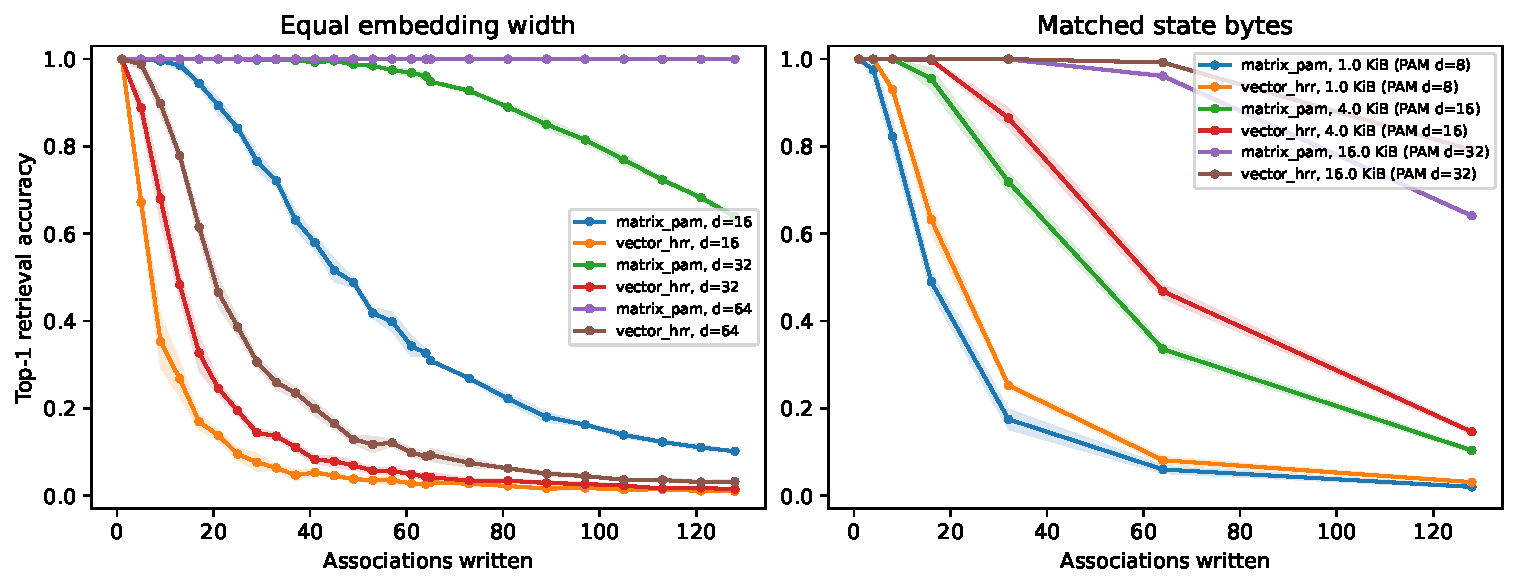
\includegraphics[width=\columnwidth]{figures/capacity.pdf}
    \caption{Equal-width and matched-state-byte binding sweeps generated from
    the versioned publication result. Shading denotes 95\% confidence
    intervals across seeds.}
    \label{fig:capacity}
  \end{figure}
}{%
  \placeholderfigure{1.05in}{Equal-width and matched-byte binding curves.
  Run the publication pipeline to generate this asset.}
}

The CPU publication sweep repeats binding, persistence, and rank across five
seeds and dimensions $16$, $32$, and $64$, and generates Figure
\ref{fig:capacity} directly from the versioned JSON artifact.  Additional
precision and trained-checkpoint replication remains required.

\section{Cross-Architecture Protocol}
\label{sec:crossarch}

Comparisons should match capability tier, numerical budget, and protocol.
The current adapters support associative and stateful measurements for \pam\
and the reference attention cache, but only stateful rank for Mamba.  The
attention adapter appends unit-norm keys and values and applies a chosen
softmax temperature; it is a reference associative store rather than a
drop-in evaluation of a trained Transformer.  The Mamba adapter inspects an
SSM state, but does not define an artificial key--value read.

\todoexp{Train or select matched checkpoints for every architecture; specify
parameter count, data, optimizer, sequence curriculum, state-byte budget,
precision, and inference implementation.  Report throughput and memory
alongside intrinsic scores.  Run LongBench, RULER, and BABILong only as a
separate behavioral layer, then test whether intrinsic failures predict
behavioral failures.}

\section{Limitations and Validity}
\label{sec:limitations}

\paragraph{Mechanism versus behavior.}
The synthetic suite can verify recurrence and expose storage dynamics.  It
cannot establish that a language model retrieves a fact in text, verbalizes
it, or reasons with it.  The language-derived filler probe still uses
untrained projections and an intrinsic score.

\paragraph{Metric interpretation.}
Relative retrieval is unsigned alignment and can exceed one.  A high effective
rank can represent useful diversity or noise; a low rank can reflect
compression rather than failure.  Results should therefore be reported as a
profile, not collapsed into an unvalidated scalar leaderboard.

\paragraph{Adapter semantics.}
The common interface does not make unlike mechanisms identical.  Attention
has a growing cache, while fixed-state systems compress history.  Some
architectures lack native associative reads.  Applicability and state cost
must accompany each score.

\paragraph{Reproducibility.}
The NumPy synthetic probes use seed 42 in the saved runs.  Layer and real-text
diagnostics can depend on initialization unless a checkpoint and all random
states are fixed.  The present results are a scaffold-quality case study, not
a final statistical evaluation.

\section{Publication Experiments}
\label{sec:future}

\todoexp{Run the implemented contrastive trained-model protocol on matched PAM,
Transformer, and Mamba checkpoints; overlay behavioral recall-versus-distance
on intrinsic curves; and compare it with persisted learned protection-gate
diagnostics for content and filler tokens.}

\todoexp{Test the proposed J-space bridge only with a reproducible
implementation of the averaged Jacobian lens: measure whether a retained
controlled fact enters a token-linked verbalizable direction, intervene on
that direction, and separate storage, workspace access, and reasoning
failures.  No such result is claimed here.}

\section{Conclusion}

We introduced a scaffold for an intrinsic neural-memory benchmark that
separates storage diagnostics from end-to-end intelligence evaluation.
Capacity, persistence, interference, effective rank, and long-distance
protocols expose distinct failure modes under controlled updates.  The \pam\
results serve only as a worked example and show why careful normalization,
capability declarations, and mechanism-versus-behavior qualifications are
necessary.  The benchmark is complementary to long-context behavioral suites
and to J-space interpretability: together, these layers could localize whether
a fact was lost in storage, unavailable to a verbalizable workspace, or
misused by downstream computation.

\section*{Reproducibility Statement}

The reference implementation is in the repository's
\texttt{memory\_probes/} package.  The values quoted here are traceable to
\texttt{logs/memory\_probes/memory\_probes\_all\_20260623\_160013.json},
\texttt{memory\_probes\_long\_context\_20260623\_160102.json},
\texttt{memory\_probes\_language\_filler\_20260623\_160106.json}, and
\texttt{memory\_probes\_rank\_text\_20260623\_160120.json}.  Core commands are
documented in \texttt{memory\_probes/README.md}.  Generated plots are
produced from versioned multi-seed JSON by
\texttt{scripts/plot\_memory\_probes\_paper.py}; the source still compiles
without those assets.

\bibliographystyle{plain}
\bibliography{references}

\end{document}
